% Confusion Matrix for Temporal DGNN
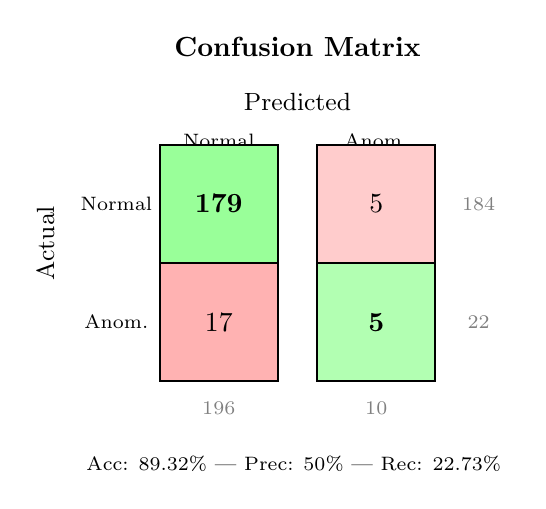
\begin{tikzpicture}[
    cell/.style={
        rectangle,
        minimum width=1.5cm,
        minimum height=1.5cm,
        draw=black,
        thick,
        font=\normalsize
    }
]

% Title
\node[font=\bfseries] at (3.5, 4.5) {Confusion Matrix};

% Labels
\node[font=\small, rotate=90] at (0.3, 2) {Actual};
\node[font=\small] at (3.5, 3.8) {Predicted};

\node[font=\scriptsize] at (2.5, 3.3) {Normal};
\node[font=\scriptsize] at (4.5, 3.3) {Anom.};
\node[font=\scriptsize] at (1.2, 2.5) {Normal};
\node[font=\scriptsize] at (1.2, 1) {Anom.};

% Cells
\node[cell, fill=green!40] at (2.5, 2.5) {\textbf{179}};
\node[cell, fill=red!20] at (4.5, 2.5) {5};
\node[cell, fill=red!30] at (2.5, 1) {17};
\node[cell, fill=green!30] at (4.5, 1) {\textbf{5}};

% Row/col totals
\node[font=\scriptsize, gray] at (5.8, 2.5) {184};
\node[font=\scriptsize, gray] at (5.8, 1) {22};
\node[font=\scriptsize, gray] at (2.5, -0.1) {196};
\node[font=\scriptsize, gray] at (4.5, -0.1) {10};

% Metrics
\node[font=\scriptsize, align=center] at (3.5, -0.8) {
    Acc: 89.32\% | Prec: 50\% | Rec: 22.73\%
};

\end{tikzpicture}
